
\documentclass[journal]{IEEEtran}

\usepackage{biblatex}


\usepackage[fleqn]{amsmath}
\usepackage{amssymb}
\usepackage{graphicx}
\usepackage{cancel}
\usepackage{tabularx}
\usepackage{algorithm}
\usepackage{algorithmic}
\usepackage{parskip}

\usepackage{bookmark}

% \usepackage{caption}
% \usepackage{subcaption}

\usepackage{subfig}
\usepackage[authordate,autocite=inline,backend=biber,sorting=nyt,natbib=true]{biblatex}
\addbibresource{citations.bib}



\graphicspath {{src/images}}
\graphicspath {{src/images/latex}}

\usepackage{hyperref}
\hypersetup{
colorlinks=false,
linkcolor=blue,
filecolor=magenta,
    urlcolor=blue,
}
\urlstyle{same}

\begin{document}

\title{Path Planning For Autonomous Vehicles}
\author{Jonathan~Dorsey  \\  \url{https://github.com/JonnyD1117/python-path-planners}}

% \IEEEmembership{Member: No Sleep Club: est. 2017}
\markboth{Journal of Graduate School Assignments March~2023}

\maketitle

\begin{abstract}
  This work introduces the problem of path planning for mobile autonomous vehicles, in static environments.It focuses on the practical context surrounding path planning such as occupancy grid maps, simultaneous localization and mapping (SLAM), and graph generation. After providing a broad overview of the general problem context, this paper surveys several of the most common and widely used planning algorithms. These algorithms include A*, Dijkstra's shortest path, Rapidly Exploring Random Trees, and Probabilistic Road Maps. Each of these algorithms has previously been the stateoftheart, in path planning, for mobile robots over the years and each continues to provide the theoretical foundational that many modern path planners are often synthesized from. This paper concludes with a case study covering the realworld performance, capabilities, and limitations for each of the aforementioned algorithms under a scenario of path planning for autonomous vehicles in known environments.
\end{abstract}

% Note that keywords are not normally used for peerreview papers.
\begin{IEEEkeywords}
	A*, Dijkstra, PRM, RRT, path planning, mobile robots, autonomous vehicles
\end{IEEEkeywords}

\IEEEpeerreviewmaketitle

\section{Introduction}

\IEEEPARstart{R}{obotics} is a broad, complex, and multifaceted field of study that integrates a wide range of technical disciplines. One of the most visible applications of robotics, in the public consciousness, is the emergence of autonomous vehicles and the advancements in technology and computing which has made it feasible. The task of automating the movement of a vehicle or robot in a safe, practical, and reliable manner is a complex endeavor that engages many tough societal and technical issues. One of the most fundamental technical challenges is the task of \textbf{path planning}. This problem is of primary importance as the creation of a feasible path through a known or unknown space is often the first of many stages in a guidance and navigation stack.

The broad objective of this paper is to survey a selection of the most popular path planners in use today, juxtapose their relative merits, and contextualize the process of constructing and implementing these algorithms in Python to test their performance. Additionally, this paper covers the post-processing of path planner waypoints into a usable continuous path for certain realworld applications.   

\section{The Path Planning Problem} 

As it applies to mobile robotics, the path planning problem can be stated as, the task of generating a feasibly traversable sequence of waypoints (aka a path) between a starting position and a target destination. The creation of this path is possibly subject to finite compute resources, a cost-function, and/or a set of system constraints. Additionally, in its' most general form, path planning allows for the inclusion of dynamics obstacles, in the environment. 

It should be immediately obvious that this definition describes a very broad class of physical environments, possible algorithms, and path generation criteria. However, with the inclusion of a few notable exceptions, most path planners that are described by the previous definition will require a solution that plans in realtime, to handle the dynamic elements within an environment. This is not always desirable, reasonable, or even realizable. Depending on the intended function and computational resources available, these assumptions often need to be relaxed and simplified to reach a feasible solution

\subsection{Offline Planning for Static Environments}

One of the most common simplifying assumptions, within the domain of path planning, is to assume that the world the mobile robot is operating within is completely static. Frequently, this assumption is sufficient to model large complex environment. This not only permits a class of faster and less resource intensive planning algorithms, but also provides a simple and reliable foundational layer that obstacle detection and avoidance algorithms can build on to handle dynamic elements in a local (instead of a global) sense, allowing simple programs to build complex behaviors together in a modular fashion instead of building large monolithic solutions. 

Additionally, static planners are frequently utilized to quantify the statistical performance of an algorithm or to understand the limitations that could arise from the application of planning in real-world edge conditions. 

As the objective of this paper is to present and compare a handful of fundamental path planning algorithms, the rest of this paper makes the assumption that path planning is occurring in a static environment.
\section{Prerequisite Concepts}

Like many other domains within the study of robotics, path planning involves the understanding and implementation of concepts borrowed from other disciplines. This section attempts to clearly and concisely present key concepts and details in hopes of anchoring the following discussion by first contextualizing some of the important tasks, principles, and assumptions that are fundamental in the design and implementation of the planners covered in this paper.

\subsection{The Mapping Problem}

One of the most fundamental requirements for any path planning system is to develop an understanding of where it is in the physical world. It would be impossible for a robot to navigate its environment without the ability to know where it currently is, the location of its final goal state, and the location of obstacles or constraints within the environment. This implies a need for the generation of an intermediate representation that a robot can utilize to localize and navigate through.  

By definition, a physical environment is the ground truth representation which we would like the robot to understand; however, this is typically impossible for all but the simplest of environments. The best that can done is to embed as much information as possible into a simplified representation of environmental features. The task of transforming sensor data into a representation that is suitable for navigation is called \textbf{mapping}.  

During the mapping process useful features, measurements, or landmarks are extracted from the environment, and structured into an often compressed and lossy representation of the ground truth. The specific data structures and algorithms used vary greatly depending on the application, the number and type of sensors available, as well as the type and speed of compute resources. These representations vary in structure, fidelity, and ease of use ranging from dense 2D/3D lidar point clouds to application specific feature extractors that can fuse several sensors together to extract the desired information. 

One of the primary tradeoffs when generating a map is the balance between simplicity, size, and data quality. More often than not, maps are chosen to be overly simple as these can achieve better performance and faster update rates than a more complex mapping which might require more computation to process and query. Even so, the objective still remains to preserve as much feature quality as possible (e.g limit measurement/environmental uncertainty) while still completing the desired task(s) within an acceptable margin. As with many things in robotics, acceptable mapping performance often is a result of correct parameterization. As such the representation for a map (or the associated data structures) can have a tremendous impact on the fundamental design and limitations concerning the underlying mechanism or efficiency for a particular path planning algorithm.

It should be noted that in the domain of mobile robots the process of mapping is generally referred to as Simultaneous Localization and Mapping (SLAM). Unlike the mapping of a room by a static observer, SLAM algorithms need to account for the location and movement of the robot while it is generating a map from its sensor data. While considered by most to be a solved problem, improvements in this field are still evolving as sensor technology (e.g. 3D Lidar Sensors...etc) and onboard computation increases further unlocking the reality of higher fidelity maps that can be generated in close to real-time. 


This brief overview has only provided the most superficial glimpse into the process of mapping for mobile robots to establish the dependency between map generation as a prerequisite to plath planning. 


\subsubsection{Dimensionality Reduction \& Discretization}

In the era of computers, map generation routinely tradeoffs quality and quantity of information for portability and efficiency in computing. This typically means that maps must be compact enough to fit into system memory or onboard storage as well as being efficient to query. To this end, even though robots exist in a three-dimensions of space, it is often sufficient to navigate the 3D world, by planning a path in a 2D projection. This technique is called \textbf{dimensionality reduction}. 

Unfortunately, even a 2D continuous map is often computationally too untractable to resolve explicitly. The most common approach to this problem, not just in robotics but also in computational mathematics, is to discretize a continuous domain into discrete grids or cells. By doing so, the computer can efficiently store and access each cell of a map with finite resources. The side-effect of discretization is an unavoidable loss/degradation of the original information.

\begin{figure}[ht]
  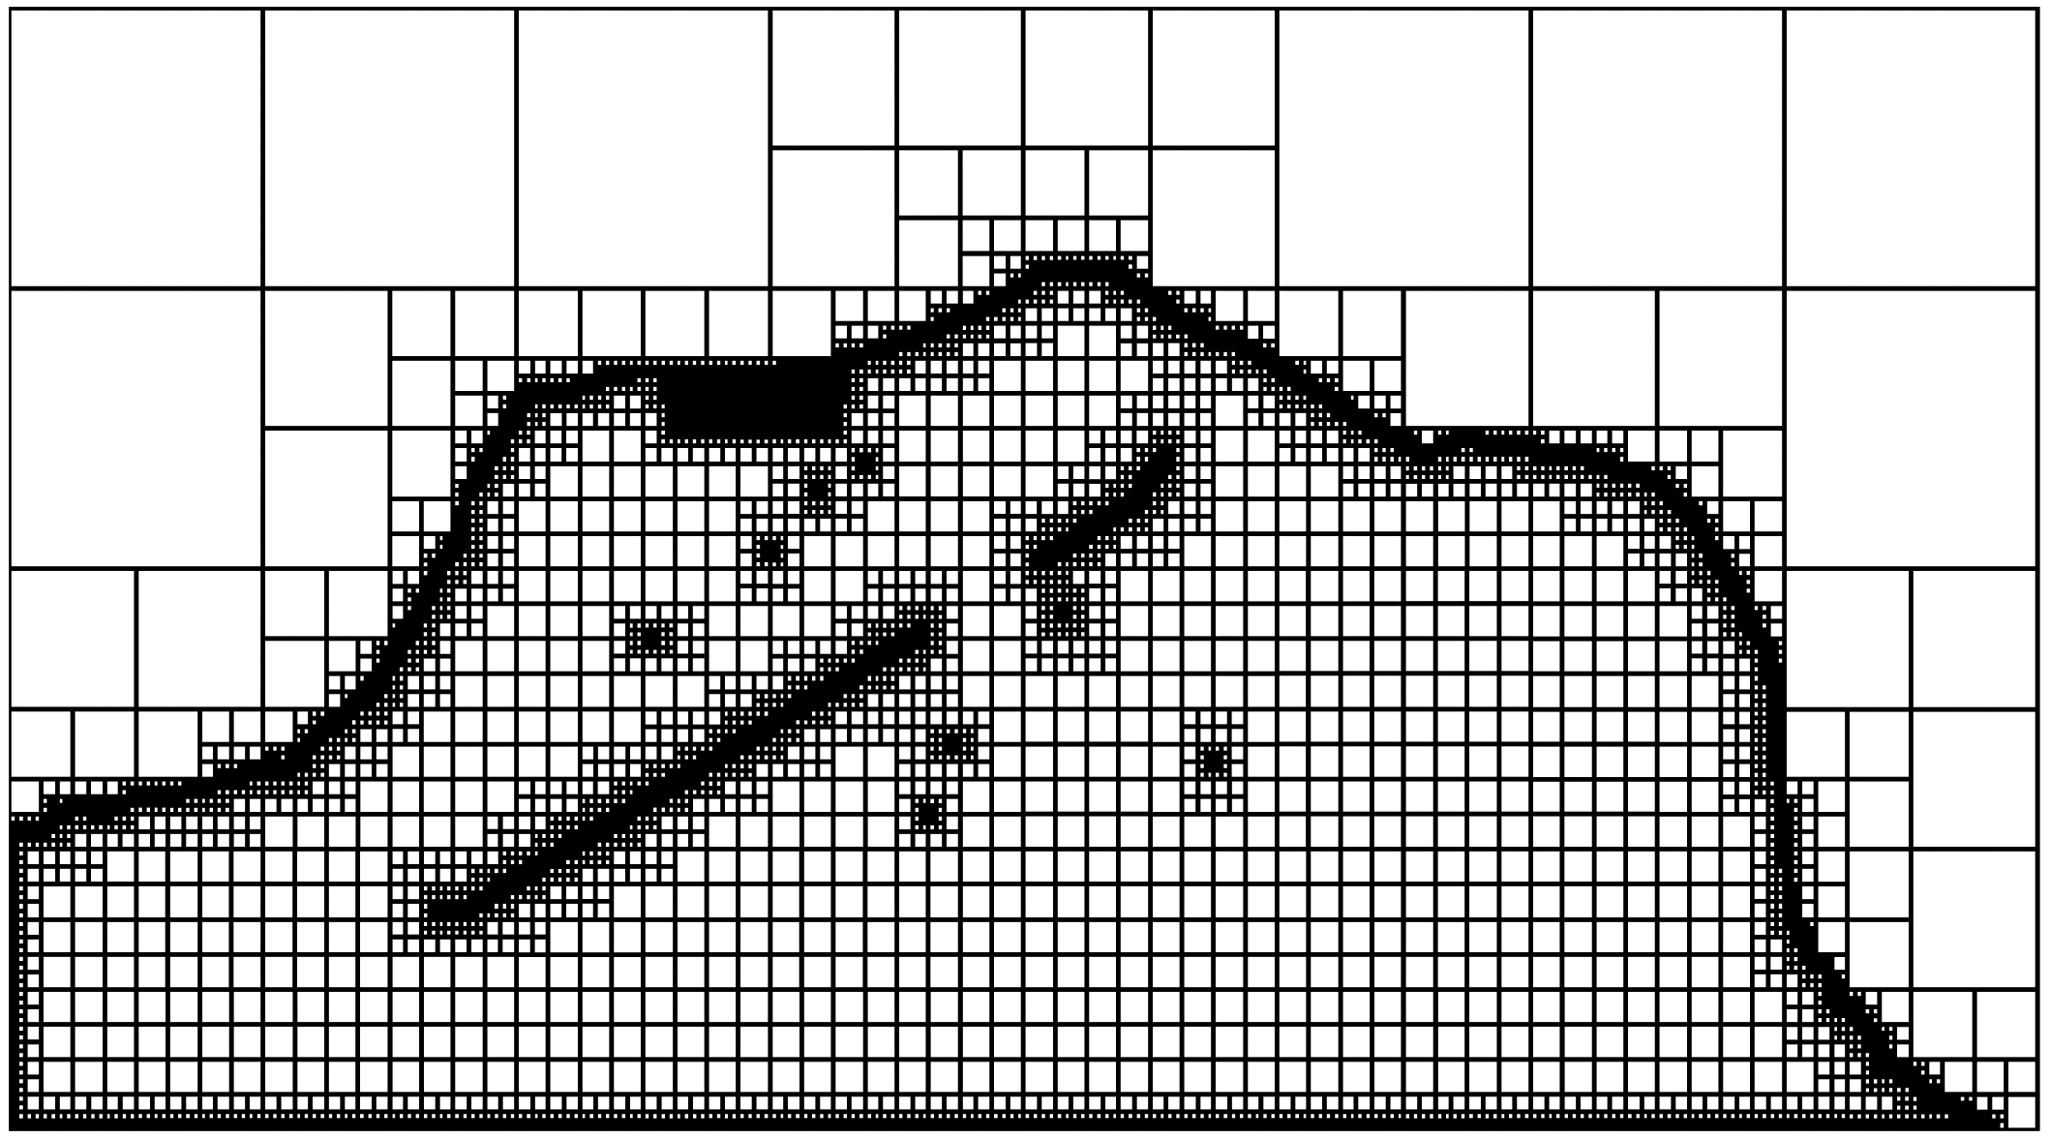
\includegraphics[width=8cm]{quadtree}
  \centering
  \label{fig:quadtree}
  \caption{Example of Quadtree Discretization}
\end{figure}

While undesirable, carefully parameterization and clever discretization methods aid in mitigating lossy behavior, or ensure that any degradation of quality is functionally insignificant to the problem at hand. There are several popular spatial discretization schemes, with the most common listed below. 

\begin{itemize}
  \item Uniform Grid
  \item Quad Tree (2D discretization)
  \item Oct Tree (3D voxelization)
  \item Delaunay Triangulation (2D or 3D Mesh generation)
\end{itemize}


Generally, the most commonly used method is a uniform discretization. This structure is intuitive, simple to understand, and fast to implement in code; however, uniform discretization is subject to the curse of dimensionality. Whenever an environment is large and requires a high resolution, uniform grids become slow to search and expensive to store. In these situations, a clever trick is to partition a space into an non-uniform grid structure using Quad or Oct trees. These data structures are built so that they will keep the grid as large as possible unless it is a region of the map that is determined to require higher resolution. 

In the case of Quad and Oct trees, recursive discretization is only performed around the perimeter of obstacles. This allows for the majority of the grid to be constructed from coarse grid cells while grid cells surrounding obstacles are finely resolved. This variable resolution enables fast generation of paths through free space while simultaneously providing highly resolved grids around obstacles so that they can be circumnavigated efficiently.

% \subsubsection{Inverse Sensor Model}

% One of the most important parts of the mapping process is the generation of map features from global knowledge or sensor data. 

% Given a uniformly discretized mapping, we still need to 

% % Now that we have talked about what a grip map is, why they are important and how they are used in mobile robotics, talk aobut how we can use a 2d Planar lidar to create one using the inverse sensor model. 
% % \subsubsection{Bresenham Line Algorithm}
% % Then... Discuss how due to the nature of the grip map being discretized we need a method to deterine which pixels should be included to create a straight line. 
% % Discretization causes aliasing (jagged edges) bresehams line algorithm allows use to draw a line between any two pixels on a screen. (used in computer graphics)
% % For grid map generation, we used bresehams line algorithm as a model of the laser beam to determine which cells of the grid map are free space and which cells are occupied. 

% There are a limited number of situations that violate this assumption; however, these counter-examples typically rely on the existance and ability to access \textbf{global} data about an environment. An common example of this occurs in video games or simulations where the position of a character, game object, or element is known \textit{a priori}. In this class of applications, a character/robot does not need to localize itself or sense its' environment, in the classical sense, as the entire world is a construction which can be queried. 


\subsubsection{SLAM}
Frequently, there exists situations where functional maps do not exist for a given environment, and they must be either preprocessed or computed on the fly by the robot as it traverses the environment \cite{thrun2005probabilistic}. The latter operation is known as \textbf{Simultaneous Localization \& Mapping} or SLAM for short. SLAM is an incredibly deep field of study with many different approaches from EKF SLAM, Graph SLAM, RGBD SLAM, and other vision based SLAM algorithms

For the purpose of this paper, it suffices to say that without a complete or partial mapping of the environment, the robot will first have to construct the map before its able to fully plan a path through the environment. While SLAM is an important area in mobile robotics, for the planners implemented in this paper, we assume that map has already been generated and has been provided to the path planner offline.

\subsubsection{Occupancy Grid Maps}

One of the most popular mapping representations is that of the \textbf{occupancy grid map} (OGM), also referred to as a probability grid map or PGM \cite{thrun2005probabilistic}. As the name implies, this map is composed of a grid; however the unique distinction of an OGM is that each cell is associated with a probability ranging from $[0, 1]$. This value indicates the probability that a grid cell is occupied. Zero indicates completely free and one indicates completely obstructed, with any value between indicating the likelihood of occupancy. 


\begin{figure}[h!]
  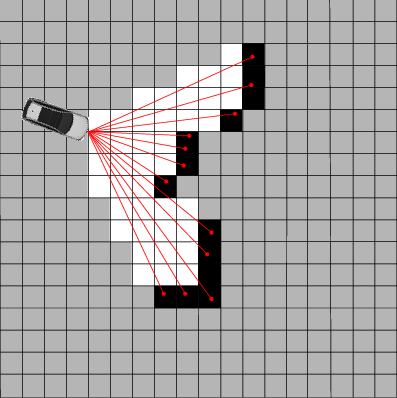
\includegraphics[width=4cm]{pgm}
  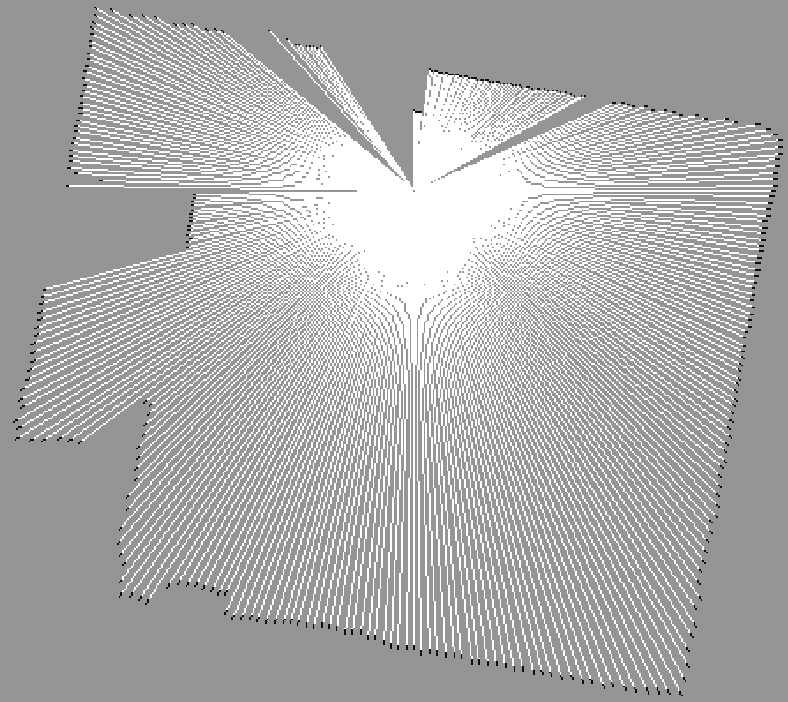
\includegraphics[width=4.5cm]{pgm_example}
  \centering
  \label{fig:grid_map}
  \caption{Occupancy Grid Map}
\end{figure}



One of the many advantages an occupancy grid map possesses is how computers store and process them. If we assume a 2D grid map with a uniform discretization, the grid map effectively becomes a grayscale picture of size $m \times n$ pixels and a resolution of $2^d-1$, where "d" is the bit depth. The similarity between occupancy grid maps and grayscale images is so striking that most grid maps are actually stored as 8-bit grayscale images within the computer. This is very practical as many programming languages have libraries that can easily read in images and are optimized to perform operations over them rapidly. The remainder of this paper assumes that every map is encoded as a occupancy grid map. 

\subsection{Graph Generation}
Graph-based planners have historically been the most popular and practical implementation for defining maps of non-trivial size. For the purposes of this paper, all of the planners that we will cover are graph-based and use some variant of a graph-like data structure (e.g. graphs or trees) \cite{gna}.

\begin{figure}[h]
  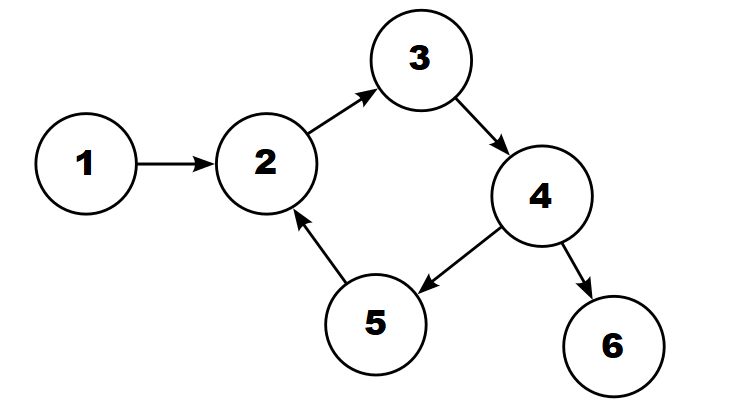
\includegraphics[width=4cm]{dgraph.png}
  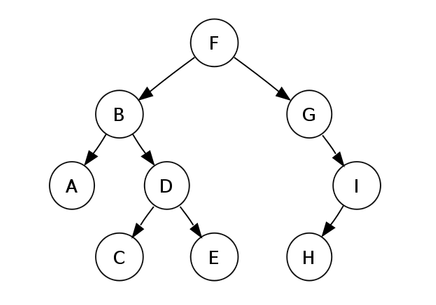
\includegraphics[width=4.5cm]{tree}
  \centering
  \label{fig:graph}
  \caption{Graph and Tree Data Structures}
\end{figure}

\subsubsection{Grid World}
One of the most common approaches to constructing a graph is the notion of directly converting each cell of an occupancy grid map into a graph node, and then applying rules for how to wire up edges between each of these nodes. When generated from a uniformly discretized grid map, this is called a \textbf{grid world}. The uniform node generation and rule-based edge connection means that this graph is intuitive and extremely simple to implement programmatically.

The two most popular connectivity rules are known as \textbf{connected-8} and \textbf{connected-4}. In connected-4, the rules that we imposes on transitioning to a new cell limit legal moves to up/down/left/right (no diagonals are permitted.) while connected-8 graphs are allowed to move one cell in any direction up/down/left/right and diagonals. 

In addition to these connectivity rules, there are two different methods concerning how obstacles can be integrated into the final graph. These two methods are \textbf{infinite edge weights} and \textbf{edge removal}. Infinite edge weighting works by guaranteeing that the shortest (aka lowest cost) path through the graph will never be through an obstacle. Since transitioning to an obstacle node will incur an infinite cost, this prevents obstacles from being included in the final path. On the other hand, the edge removal method simply removes all edges that would connect to an obstacle node, in the graph. This method works by literally making it impossible for the planner to traverse obstacles as they have all been removed from the graph. In the case of most algorithms used for static environments, this process of handling obstacle nodes is typically static and preprocessed before the robot begins navigating within the environment.

\begin{figure}[t]
  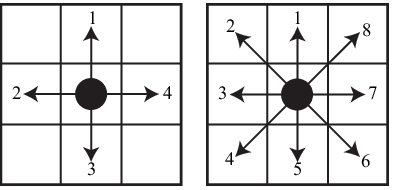
\includegraphics[width=8cm]{connectivity}
  \centering
  \label{fig:connectivity}
  \caption{Connected-4 \& Connected-8}
\end{figure}

\subsubsection{Random Sampling}

One of the downsides of grid world search graphs is the node density. By definition, every pixel of the occupancy grid map could represent a free cell, and is subject to the curse of dimensionality as the size of the map increases. To address this scaling problem, a popular technique is to employ \textbf{random sampling}. This approach is based on the concept of Monte Carlo methods, where a uniformly sampled map is used to create nodes in the graph \cite{montecarlo}. 

In principle, in the limit as the number of samples approaches infinity, we can guarantee the convergence of our path planner to the globally optimal path (if it exists). In practice, sampling-based methods can possess an order of magnitude fewer nodes while still providing enough spatial coverage at a high enough sample density to produce a feasible path through the environment that is trending towards the global optimal path. An excellent example of this is shown the in probabilistic road maps algorithm. 

\subsubsection{Binary Obstacle Inflation}

One of the pitfalls of using occupancy grid maps as the basis for the search graph is that each cell is effectively a pixel in an image. Depending on the density of our sensor coverage, there is a non-zero chance that paths through the environment that are only a single pixel wide exist. This is a problem for our robot if it happens to be larger than the adjusted real world scale of the pixel. This is almost always the case. 

To prevent situations like this from occurring and generating paths through infeasible regions of the map, we can apply a technique known as an \texbf{binary obstacle inflation}. This very simple technique artificially scales up every obstacle pixel in the scene take up more space than the actual sensor reading indicated. The result of this inflation is that sensor noise is usually absorbed into these inflated obstacles. Additionally, this technique provides a sort of poor-mans approach to prevent the phenomenon of "wall-hugging". In simple implementations of path planner, the planner does not have a concept of "robot size". This means that the planner will attempt to make the shortest path between two points, even if that path is infeasible for the robot to traverse. This is demonstrated as a sort of behavior where the path generated hugs walls in the environment to attempt reduce the distance (total cost) of the path. By applying an appropriately sized inflation layer, we can guarantee that the path between points, accounts for the physical footprint of the robot. While nifty, there are more sophisticated techniques based on applying cost gradients as a function of the distance away from an obstacle/wall. The cost gradient incentivizes the planner to prefer cells that are farther away from walls; however, this requires more postprocessing of a map before being fed into the planner.
\section{Path Planning}

In the domain of robotics, there are hundreds if not thousands of different path planning implementations some of which present totally new formulations for planning but most present incremental improvements that decrease the computational resources, or optimize some custome metric. The goal of this paper is to present a handful of the most popular (and historically important) path planners that have made a significant impact in robotics and have become defacto standard benchmarks against which all other planning algorithms compare their performance. 

This paper will cover A*, RRT, PRM, and Dijkstra's Shortest Path. Each of these algorithms is graph-based in so much as they utilize a graph or tree as the data structure from which the algorithm will attempt to generate the shortest path. While algorithms like A* and Dijkstra typically can be given a preexisting graph to traverse, algorithms like RRT and PRM implement a type of Monte Carlo random sampling to generate the graph/tree that they traverse, later after the path generation phase of the planner.  This section will cover each of the aforementioned algorithms in broad strokes, describing the general construction and planning mechanism(s) at play.

\subsection{Global vs Local Planners}

Before diving into the details of each planner, it is important to clear up the role of these planners and how this role effects the type of planning being performed in the system. Planners can generally be categorized as either \textbf{global} and \textbf{local}.  

A global planner provides an idealized "global" path between the starting location and the target destination. Typically this plan is optimizing some metric(s) such as shortest distance, curvature constraints, and/or static object avoidance. In a perfect world, an autonomous robot/vehicle would only require a global planner and a means of localizing itself (from sensor measurements); however, dynamic/uncertain obstacles coupled with imperfect sensing, mapping, and localization require robots to be more robust to uncertainty. The planning algorithms shown in the paper are all examples of global planners, as we have already made the assumption that the environment is static. 

To combat environmental uncertainty, roboticists developed the idea of local planners. Functionally, local planners use onboard sensor measurements to account for uncertainties in the global path in realtime. This is accomplished by planning deviations from the global path to maintain feasibility and to remain unobstructed. Additionally, local planners can include computation to smooth the global path and provide waypoints to the control system. However, these planners are more than just post-processing of the global path in so much as they need to be aware of the pose, dynamics, kinematics, constraints, and sensor inputs of the robot/vehicle.

\subsection{Path vs Motion Planning}
Frequently, the terminology of path planning is conflated with that of motion planning. While related, these concepts are very different and each solves a different problem. In path planning, the objective is to find the path through an environment that optimizes some metric and obeys specified constraints. Typically this metric is distance or cost and the constraint is to maintain a feasible and obstacle free path between the starting and ending points. 

Motion planning, on the other hand, uses path planning as an input to determine how the path should be traversed through time. This means not only planning the position of the path (e.g path planning) but also planning the velocity, acceleration, and often the jerk of a robot as it follows the given path. Almost always, motion planning requires the ability to compute derivatives of the path position. 

\subsection{Planning Algorithms}

The first category of planning algorithms are so-called \textbf{Graph-Search}. The primary mechanism these planners employ is to construct a graph from a map. Once this has been achieved, different algorithms, heuristics, and operations can be applied to the graph to endeavor to find the shortest path between two nodes that exist in that graph. Occupancy grid maps are ideal for the such path planners in that it is trivial to translate the grid map into a graph data structure by assuming that every pixel in the grid map is node in the graph, and then formulate the connectivity rules as desired (see \textbf{connected-4} or \textbf{connected-8} above). 

\subsubsection{Dijstra's Shortest Path}
The predecessor of almost all graph-search planners is Dijkstra's shortest path. This algorithm was invented by Dutch mathematician Edsger Dijkstra in Norway in 1956. It implements a type of breadth-first search that will traverse an undirected graph, until it has found the shortest route between two nodes within the graph. 

The implementation found in this paper for Dijkstra's algorithm uses an occupancy grid map to generate a dense graph. Cells in the map that have an occupancy value over a certain threshold are assumed to be occupied. The algorithm works by computing the cost of the current node, and then determining the total cost of each neighbor from the current node. The neighbor with the least cost is expanded in the same way until either the entire graph has been explored or the path from the start and end nodes has been determined. See algorithm for more details.

While this algorithm is simple and guaranteed to find the shortest path in the graph, assuming it exists, it cannot predict the efficiency of how well it is at finding the shortest path. This is predominately attributable to the fact that the algorithm is a generalization of a breadth-first search, blindly expanding every node closest to it without any concern to focus the direction of the search towards more likely paths (e.g. in the direction of the goal state).

% 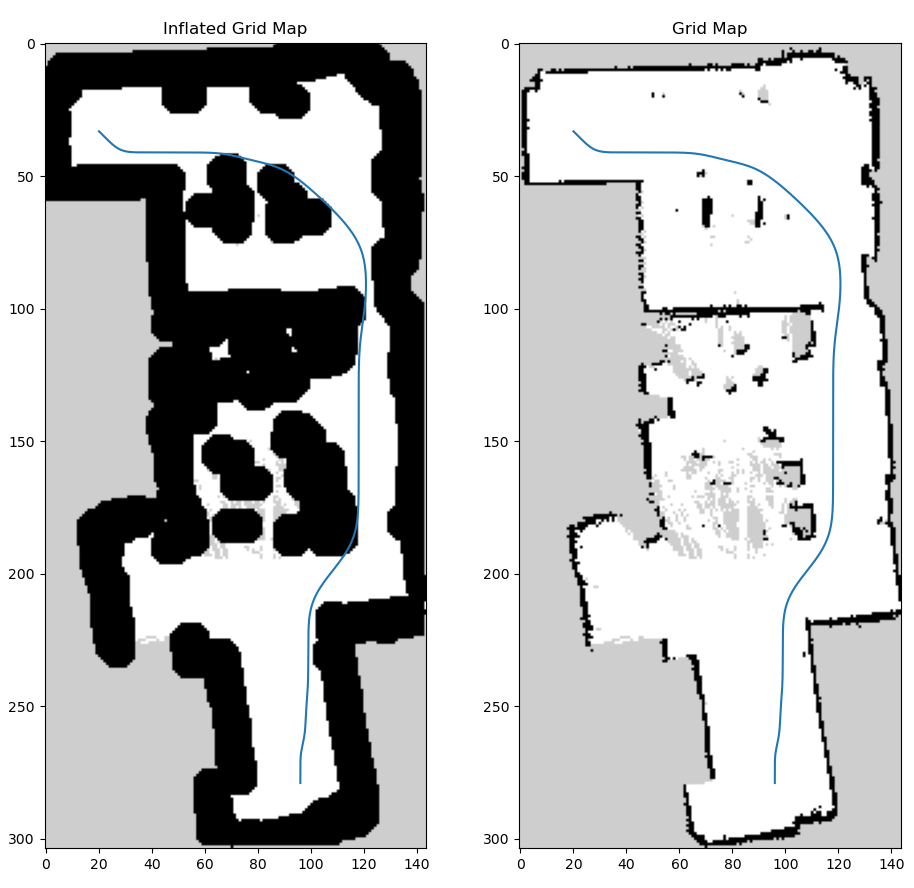
\includegraphics[scale=.3]{dijkstra.png}

% \subsection{Dijkstra Shortest Path}
\label{Dijkstra}
\begin{algorithm}
  \caption{Dijkstra's Shortest Path}
  \begin{algorithmic}[h!]
  % \renewcommand{\algorithmicrequire}{\textbf{Input: Graph, startNode, targetNode}}
  % \renewcommand{\algorithmicensure}{\textbf{Output: Path}}
   \FOR { node in Graph }
   \STATE $\text{node.score} := \infty$
   \STATE $\text{node.visted} := \text{false}$
   \ENDFOR

   \\ \textit{Solve Graph} :
   \STATE $\text{starNode.score} := 0$
   \WHILE { ( true ) }
  \STATE $\text{currentNode} := \text{nodeWithLowestScore(Graph)}$
  \STATE $\text{currentNode.visted} := \text{true}$

    \FOR { ( node in currentNode.neighbors ) }
    \IF{ ( $\text{node.visited} == \text{false}$ ) }
    \STATE $\text{newScore} := \text{calculateScore(currentNode, node)}$
    \IF{ ( $\text{newScore} < \text{node.score}$ ) }
    \STATE  $\text{node.score} := \text{newScore}$
    \STATE  $\text{node.routeToNode} := \text{currentNode}$
    \ENDIF
    \ENDIF
    \ENDFOR
    \\
    \\ \textit{Return Path} :
    \IF{ ( currentNode == targetNode ) }
    \RETURN build{Path(targetNode)}
    \ENDIF

    \\
    \\ \textit{Raise Error if No Path is Found} :

    \IF{nodeWithLowestScore(graph).score == $\infty$}
    \RETURN ERROR: No Path Found
    \ENDIF

   \ENDWHILE

  \end{algorithmic} 
  \end{algorithm}



\begin{figure}[h!]
    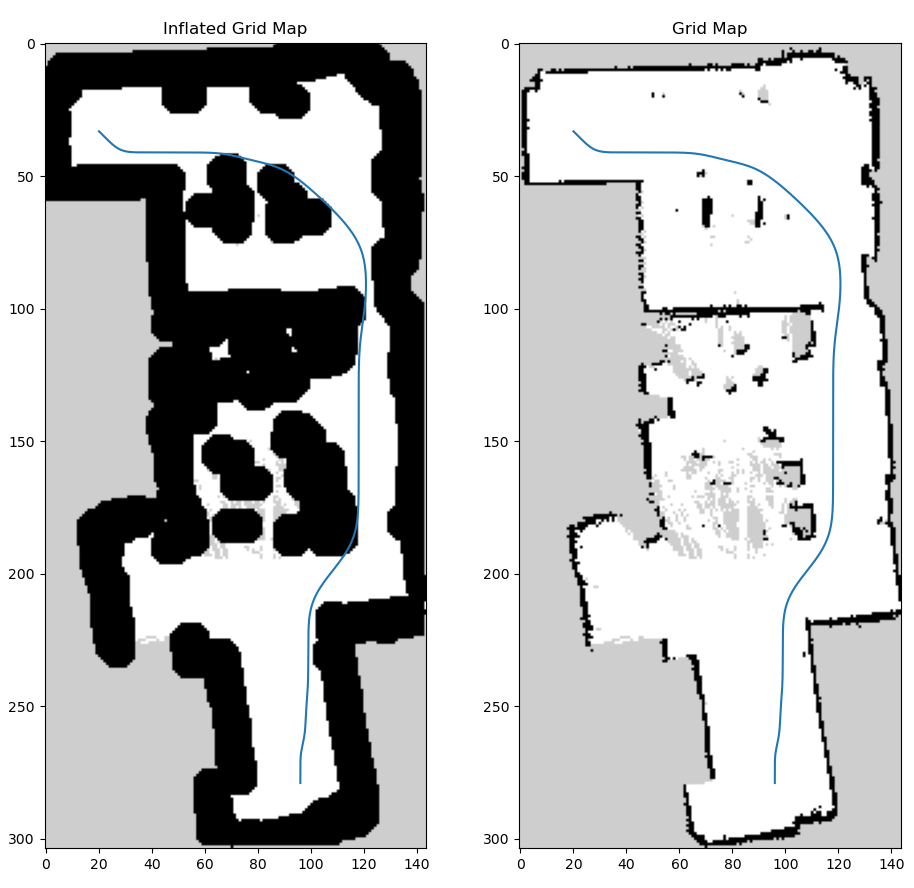
\includegraphics[width=8cm]{dijkstra}
    \centering
    \label{fig:Dijkstra}
    \caption{Dijkstra Algorithm in SLAM generate Map}
\end{figure}


\subsubsection{A*}

The A* algorithm was developed at the Stanford Research Institute in 1968, for the historically significant robot Shakey, being used in some of the earliest pioneering research into mobile robotics. It is both the literal and conceptual successor to Dijkstra's algorithm. Both implement a graph-search; however, the primary improvement of A* is the addition of a heuristic that improves the ability of the search algorithm to focus on expanding nodes in the direction of the goal state.  

Unlike Dijkstra's algorithm, the addition of a heuristic provides the planner with the ability to preferentially search in a given direction and will traverse nodes that are more likely to be approaching the goal node fom the starting node. So long as the heuristic is quick to compute and admissible (an exact or under estimate of the actual distance to the goal node), we can use a search heuristic to drastically improve the planners convergence rate.

A* is extremely similar to Dijkstra's algorithm described above. The key difference is how A* computes the cost of getting to the current node, and then computes the cost of traversing to each neighboring node plus the addition of a heuristic cost from each neighbor to the goal state. The inclusion of a heuristic cost allows A* to preferentially choose to visit neighbors that are closer to the goal state by choosing the neighbor with the lowest combined current plus heuristic cost. See algorithm for more details.

\label{A*}
\begin{algorithm}
  \caption{A* Heuristic Search}
  \begin{algorithmic}[1]
   \FOR { ( $\text{node in Graph}$ ) }
    \STATE $\text{node.gScore} := \infty$
    \STATE $\text{node.fScore} := \infty$
    \STATE $\text{node.visted} := \text{false}$
   \ENDFOR

   \textit{Solve Graph} :
   \STATE $\text{starNode.gScore} := 0$
   \STATE $\text{starNode.fScore} := 0$
   \WHILE { ( true ) }
  \STATE $\text{currentNode} := \text{nodeWithLowestScore(Graph)}$
  \STATE $\text{currentNode.visted} := \text{true}$

    \FOR { ( node in currentNode.neighbors ) }
    \IF{ ( $\text{node.visited} == \text{false}$ ) }
    \STATE $\text{newScore} := \text{calcScore(currentNode, node)}$
    \IF{ ( $\text{newScore} < \text{node.g}$ ) }
    \STATE  $\text{node.gScore} := \text{newScore}$
    \STATE  $\text{node.fScore} := \text{newScore} + \text{calcHeuristic(nextNode, targetNode)}$
    \STATE  $\text{node.routeToNode} := \text{currentNode}$
    \ENDIF
    \ENDIF
    \ENDFOR
    
    \\ \textit{Return Path} :
    \IF{ ( currentNode == targetNode ) }
    \RETURN build{Path(targetNode)}
    \ENDIF

    
    \\ \textit{Raise Error if No Path is Found} :

    \IF{nodeWithLowestScore(graph).score == $\infty$}
    \RETURN ERROR: No Path Found
    \ENDIF

   \ENDWHILE

  \end{algorithmic} 
  \end{algorithm}

A* has made a tremendous impact on the world of robotics and is today the defacto standard for simple path planning tasks. Unfortunately, both A* and Dijkstra suffer from the necessity to generate a graph of the environment. As previously mentioned, this usually involves the conversion of a grid map into graph. While not always an issue, the dimension of the grid map corresponds to the need to generate a larger search graph, which requires either algorithm to spend more time to compute the shortest path. Unlike Dijkstra's, the heuristic driven nature of A* also means that it is typically far more efficient of a search than Dijkstra's algorithm over the same search graph. 

% 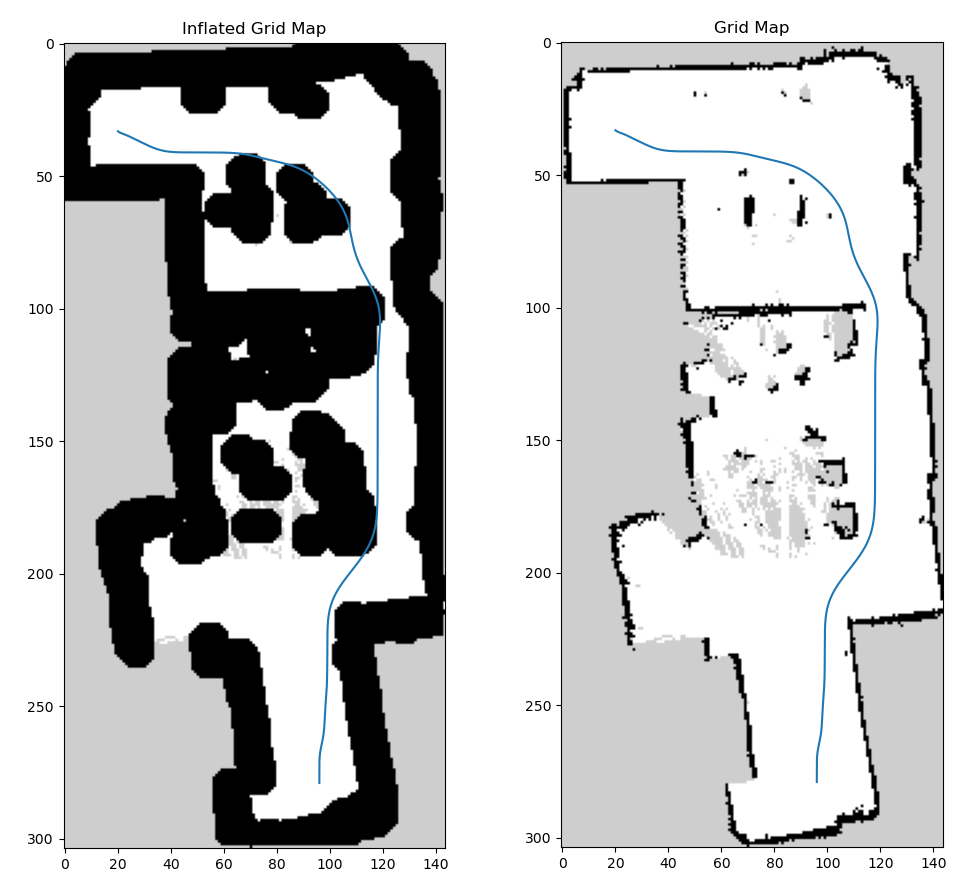
\includegraphics[scale=.3]{astar.png}

\begin{figure}[h!]
    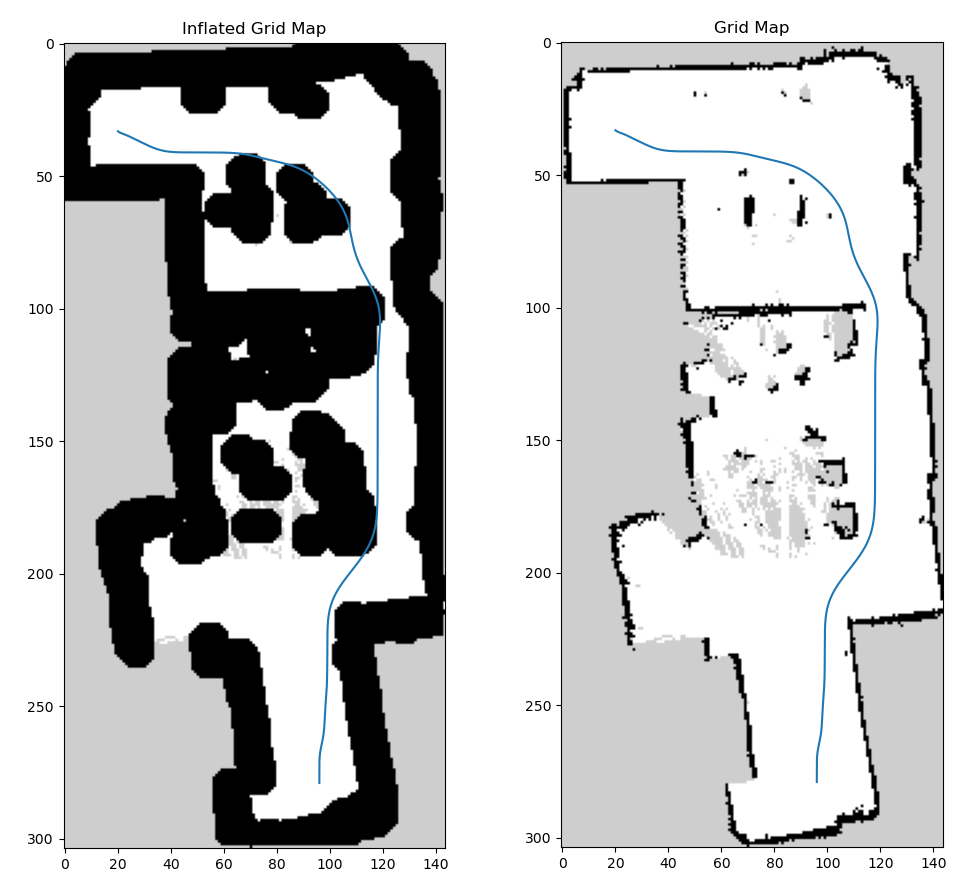
\includegraphics[width=8cm]{astar}
    \centering
    \label{fig:Astar}
    \caption{A Star}
  \end{figure}

\subsubsection{Probabilistic Road Maps}

While graph-search planners have been popular and practical historically, these methods like Dijkstra's and A* can only be as efficient as the size, resolution, and connectivity of their graph permits. Depending on how these graphs were generated, they often suffer from the inability to efficiently scale as the size of a given map increases, leading to unacceptable latency and computation times, known as the curse of dimensionality.

To address the problem of high graph densities, the algorithm Probabilistic Road Maps (PRM) was developed. PRM has two main stages; graph creation via random sampling, and path computation by directly applying Dijkstra's algorithm. The broad objective of PRM is to decrease the density of the search-graph by applying uniform sampling as the mechanism for generating graph nodes within the map. The compromise this method makes is the reduction of graph generation and graph traversal times in exchange for a lower fidelity map that is no longer pixel accurate to the map.

PRM works by randomly selecting a number of points within the domain of the map. It will first check whether or not the randomly selected point is an obstacle. If the sample is contained within an obstacle, the algorithm will redraw random samples until it finds a point that is \textit{free}. This point is then added to an every growing graph, so long as the edge connecting this new node and the previous nodes in the graph do not intersect obstacles. Once this has been performed for a sufficient number of random samples, the graph or 'roadmap' now exists. The second phase of the algorithm merely selects a starting and target nodes, in the graph and applying a graph-search algorithm between those two endpoints.

This technique is not only faster for the graph generation portion of the algorithm, but since the graph is generates is typically over an order of magnitude less dense than an equivalent grid map based graph, finding the shortest path between two points on this "sampled" graph results in significantly faster graph traversal. It should be noted that unlike the other methods, PRM is only optimal within the limit as the number of samples becomes infinite. This means that unlike A* traversing a dense grid-based graph, PRM with a finite sample size is unlikely to find the optimally shortest path; however it does provide a locally optimal path across its sampled-graph. This behavior demonstrates how PRM needs to be tuned to its targeted application for effective results.  

\label{Probalistic Road Maps}
\begin{algorithm}
  \caption{Roadmap Construction}
  \begin{algorithmic}[1]

  \renewcommand{\algorithmicrequire}{\textbf{Input:} }
  \renewcommand{\algorithmicensure}{\textbf{Output:} }
  \REQUIRE 
    \text{    n: number of nodes in roadmap} \linebreak
    \text{    k: number of closest neighbors to examine for each configuration} \linebreak

  % \textbf{Output:} \linebreak
  \ENSURE  \linebreak
    \text{    A roadmap G = (V, E)} \linebreak

  \hrulefill 

  \STATE \text{$V \leftarrow \emptyset$}
  \STATE \text{$E \leftarrow \emptyset$}

   \WHILE { $\lvert V \rvert < n$ }

    \STATE \textbf{repeat}
    \STATE $\text{     q} \leftarrow \text{random sample from Configuration Space } \mathcal{Q}$
    \STATE \textbf{until} \text{q is collision-free}
    \STATE $V \leftarrow V \cup \text{\{q\}}$
   \ENDWHILE
   \FOR {  $\textbf{all } \text{q} \in \text{V}$  }
   \STATE $N_q \leftarrow \text{the k nearest neighbors of q from V by \textit{dist}}$
    \FOR { $\textbf{all } q^{\prime} \in N_q$  }
    \IF { ($\text{q, } q^{\prime}) \notin \text{E \textbf{and }} \Delta(\text{q, } q^{\prime}) \ne 0$ }
    \STATE $\text{E} \leftarrow \text{E } \cup \{ ($\text{q, } q^{\prime}) \}$
    \ENDIF
    \ENDFOR

   \ENDFOR

  \end{algorithmic} 
  \end{algorithm}

% 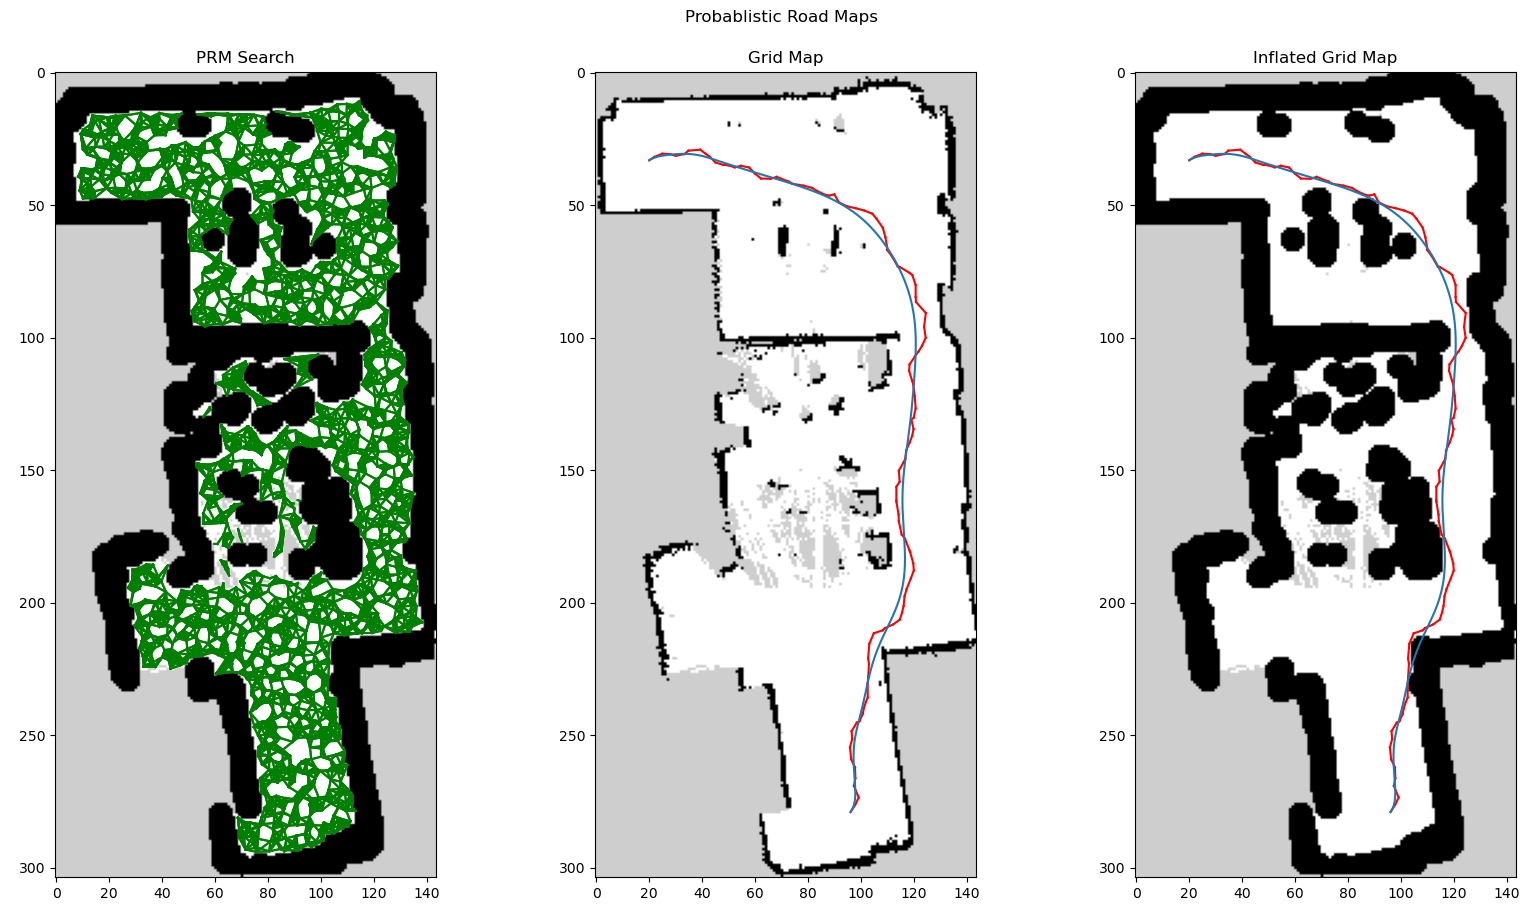
\includegraphics[scale=.23]{probablistic_road_map.png}
\begin{figure}[h!]
    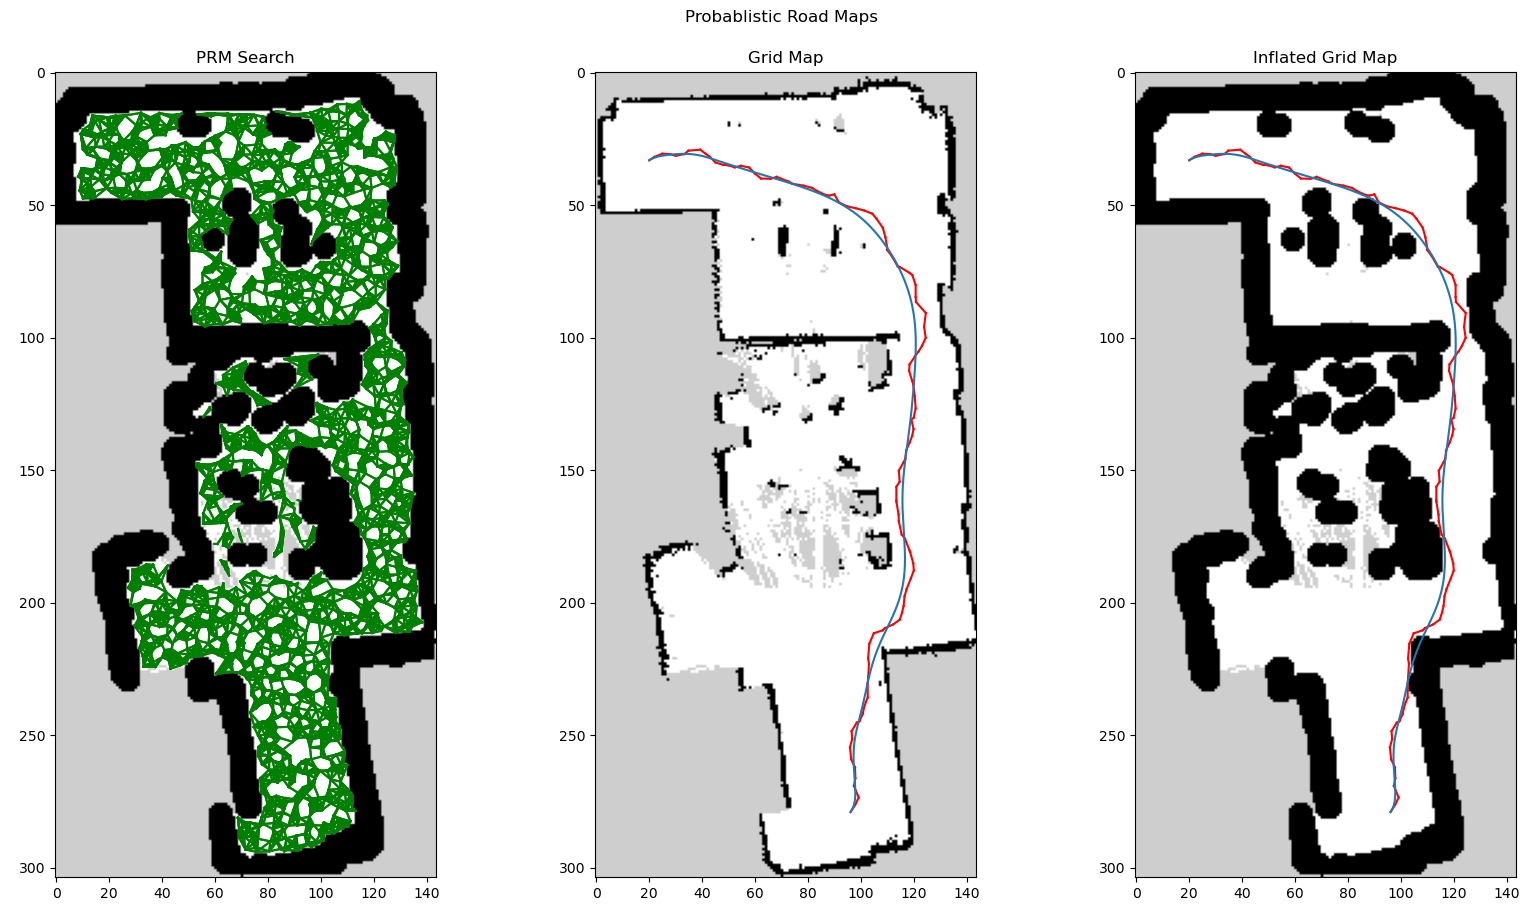
\includegraphics[width=8cm]{probablistic_road_map}
    \centering
    \label{fig:PRM}
    \caption{Probabilistic Road Maps}
  \end{figure}

\subsubsection{Rapidly Exploring Random Trees}

Similar to PRM, Rapidly Exploring Random Trees (RRT), also attempts to leverage random sampling to improve the sample efficiently and reduce the graph generation time. The primary difference between PRM and RRT is their data structures and how additional nodes are inserted into this data structure. While PRM utilizes a graph, the RRT class of algorithms use a tree structure. Tree structures possess several benefits but also impose several constraints on the representation of the map that these algorithms generate. 

The most useful aspect of using a tree is the simplicity in determining the final path. Unlike all of the graph-based methods that require iteratively searching over a large portion of nodes in the graph to determine the shortest path, a tree structure is a very simple structure that lends itself to recursive solutions. Since unlike a node in a graph, a node in a tree can only possess one predecessor, one need only begin at the final target node and recursively make a list of each predecessor node, until the starting node is reached.

Like PRM, RRT will randomly sample its map, check that these random points are not obstacles in the map (resample if true) and then create a tree by tieing that random point into the near node of the tree, by taking a step of size $\DeltaS$ towards the random point, from its closest node on tree. At this new location, it will create a new node that is parented to the nearest neighbor previously mentioned. 


% Similar to PRM, RRT is not guaranteed to find the shortest path between two nodes even in the limit as the number of samples trends towards infinitely sample the map. Unlike PRThis is due to the static nature of the tree generation. 

\label{RRT}
\begin{algorithm}
  \caption{RRT Construction}
  \begin{algorithmic}[1]

  \renewcommand{\algorithmicrequire}{\textbf{Input:} }
  \renewcommand{\algorithmicensure}{\textbf{Output:} }
  \REQUIRE 
    \text{    $q_0$:the configuration where the tree is rooted} \linebreak
    \text{    n: the number of attempts to expand the tree } \linebreak

  \ENSURE  \linebreak
    \text{    A tree T = (V, E) that is rooted at $q_0$ and has $\le $ n configurations } \linebreak

  \hrulefill 

  \STATE \text{$V \leftarrow \{q_0\}$}
  \STATE \text{$E \leftarrow \emptyset$}

  \FOR {  i = 1 to n  }
  \STATE $q_{rand} \leftarrow$ a randomly chosen free configuration
  \STATE $q_{near} \leftarrow$ closest neighbor of q in T
  \STATE $q_{new} \leftarrow$ node a dist $\Delta S$ from $q_{near}$ to $q_{rand}$
    \IF { $q_{new}$ is collision-free }
      \STATE V $\leftarrow$ V $\cup$ \{$q_{new}$\}
      \STATE E $\leftarrow$ E $\cup$ \{($q_{near}$, $q_{new}$ )\}
      \RETURN $q_{new}$
    \ENDIF
    \RETURN 0
  \ENDFOR

  \end{algorithmic} 
  \end{algorithm}
\section{Path Smoothing}
It should be noted that all of the path planners covered, in this paper, have generated piece-wise linear paths between two discrete points in space. With the exception of a path that only contains two points, the shortest path generated by these planners will always be discontinuous. The nature of this discontinuity is rooted in the discretization applied earlier throughout these planners. Unfortunately, while discretized paths are computationally desirable, they often are incompatible with the robotics system that will use the planners path.

\begin{figure}[h]
    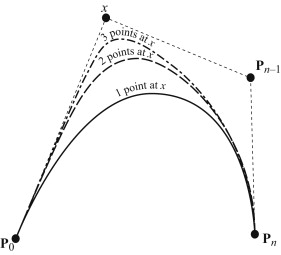
\includegraphics[width=4cm]{cubic_bezier}
    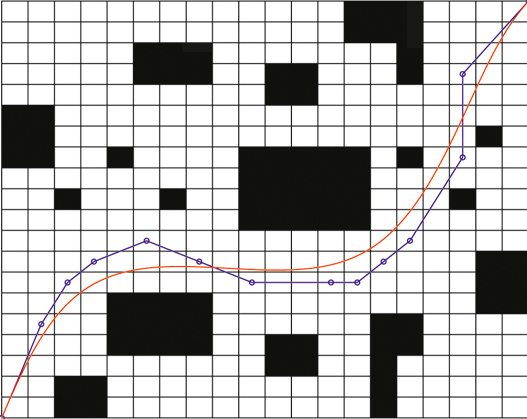
\includegraphics[width=4.5cm]{bezier_path_smoothing}
    \centering
    \label{fig:bezier}
    \caption{Cubic Bezier}
  \end{figure}

The most obvious reason for such an incompatibility is the requirement for continuous inputs into a controller, state estimator, or other component which are formulated under the assumption of continuous inputs. Secondly, even for discrete systems, it is often more desirable to generate waypoints, for the robot to track, at a much higher sampling frequency, than is practicable to produce with the planner directly. This is especially true when refining the discretization of the map to a sufficient waypoint frequency would make global path planning through the environment untractable.

This need leads to the need for the raw outputs of these planners to be post-processed via a path smoothing algorithm. As alluded to above, in this paper, the reason for smoothing the outputs of the planner come from desiring a frequency between waypoints.

\subsection{Bezier Path Smoothing}
One of the most simple and straight forward methods for path smoothing is that of Bezier curves. While the derivation of Bezier curves is beyond the scope of this paper, sufficed to say that this technique is very effective for quickly computing a curve from the planner output, that is effectively infinitely resolvable.

\subsubsection{Bezier Curve Formulation}
The formulation of a Bezier curve is the based on the three following equations. 

\begin{equation}
    \left(\begin{array}{l}
    n \\
    i
    \end{array}\right)=\frac{n !}{i !(n-1) !}
\end{equation}

\begin{equation}
    B_{i, n}(t)=\left(\begin{array}{c}
    n \\
    i
    \end{array}\right) t^i(1-t)^{n-i}
\end{equation}

\begin{equation}
    C(t)=\sum_{i=0}^n P_i B_{i, n}(t)
\end{equation}

Where $P_i$ is the point at index $i$ from output of the planner which is of length $n$ and where $B_{i, n}$ is formula for a Bernstein polynomial. 

As with the mathematical formulation of the Bezier curve, the implementation of the Bezier,in code, is very direct and straightforward. 

% \begin{figure}[h!]
%     % 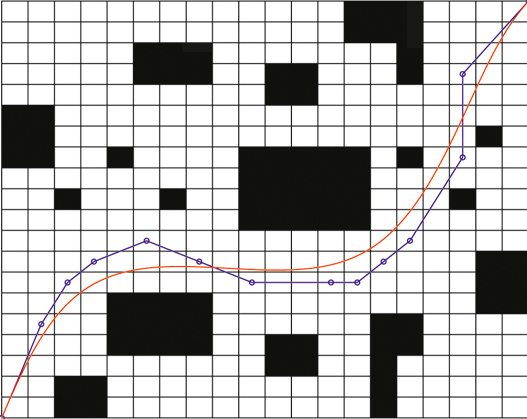
\includegraphics[width=4cm]{bezier_path_smoothing}
%     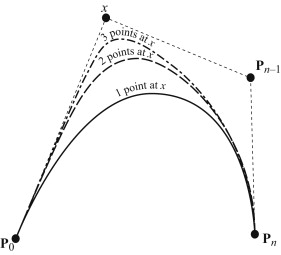
\includegraphics[width=4cm]{cubic_bezier}
%     \centering
%     \label{fig:Bezier_Curves}
%     \caption{Bezier Path Smoothing}
% \end{figure}  


\subsubsection{Limitation of Bezier Curves}
Unless the length of the planner output is exceeding large, Bezier curves tend be a quick to compute path smoothing algorithm that is very effective for many applications including simple robotic environments or in video games. Unfortunately, the primary drawback of Bezier curves in robotics, is the inability to directly model system or environmental information into the path smoothing process. In the domain of robotics, this typically manifests as the inability to apply custom constraints or guarantee feasibility of the final smoothed path.  

While guaranteeing feasibility or respecting applied constraints, might be of little meaningful importance in an application like video games, where the goal is to be good enough while using up the least compute resources, in robotics, obeying constraints and feasibility requirements is a very real necessity.

While not ideal, the Bezier curves does often work for robots in simple environments. Acknowledging this short-coming, this paper, has applied Bezier path smoothing to all of the path planner outputs as a means of quickly and consistently generating a smooth output path.


\subsection{Optimization Based Path Smoothing}
The other predominate class of path smoothing algorithms comes in the form of optimization based methods. Unlike Bezier smoothing, these methods work on the principle of minimizing some cost function associated with the points output by the planner. The strength of optimization-based methods involve the natural ability to define and apply constraints to that the solution of the optimizer must obey. For path smoothing, this translates into the ability for these methods to intuitively constraints such that the smoothed path will never intersect with static obstacles in the environment, or violate feasibility by generating a path whose curvature is impossible for the robot to track.

Generally, this method is far more computationally expensive to realize than that of Bezier curves; however, the benefits that it brings are often significant enough for specialize high efficiency variants to be designed specially for real-time robotic applications. 

\subsubsection{Timed-Elastic Band}
One such method that has been specially adapted for the use with car-like robots (e.g. autonomous vehicles), is that of \textbf{Timed-Elastic Band} optimization. This problem is formulated mathematical below.  

\begin{equation}
    \begin{array}{l}
    \min _{\mathcal{B}} \sum_{k=1}^{n-1} \Delta T_k^2 \quad(\mathrm{NLP}) \\
    \text { subject to } \\
    \mathbf{s}_1=\mathbf{s}_c, \mathbf{s}_n=\mathbf{s} f, 0 \leq \Delta T_k \leq \Delta T_{\max }, \\
    \mathbf{h}_k\left(\mathbf{s}_{k+1}, \mathbf{s}_k\right)=0, \quad \tilde{r}_k\left(\mathbf{s}_{k+1}, \mathbf{s}_k\right) \geq 0, \\
    \mathbf{o}_k\left(\mathbf{s}_k\right) \geq 0, \\
    \nu_k\left(\mathbf{s}_{k+1}, \mathbf{s}_k, \Delta T_k\right) \geq 0, \quad(k=1,2, \ldots, n-1) \\
    \alpha_k\left(\mathbf{s}_{k+2}, \mathbf{s}_{k+1}, \mathbf{s}_k, \Delta T_{k+1}, \Delta T_k\right) \geq 0,(k=2,3, \ldots, n-2) \\
    \alpha_1\left(\mathbf{s}_2, \mathbf{s}_1, \Delta T_1\right) \geq 0, \quad \alpha_n\left(\mathbf{s}_n, \mathbf{s}_{n-1}, \Delta T_{n-1}\right) \geq 0 .
    \end{array}
    \end{equation}

The advantage of this algorithm is that it incorporates a standard vehicle model and produces locally optimal paths. The downside of this method is that it is required to be run online, very similarly to the implementation of Model Predictive Control (MPC).




\section{Autonomous Vehicle Case Study}

Since the intended application for the planners covered in this paper are for use with autonomous vehicles, it is only appropriate to investigate how these planners actually perform in practice and to compare their quantitative differences.

\subsection{Scenario}
The scenario we will use is taken from a concurrent research project within our lab to quantify the differences in performance between several control schemes that require an autonomous vehicle to navigate through a non-trivial environment. Since the objective of that project is to compare the relative performance between different controllers over the same path, this scenario only requires a static environment to ensure continuity between test runs using the different controllers and is the perfect candidate for testing the planners discussed above.

Unlike testing a control system, testing offline path planners can be done completely in simulation under the assumption that the input map is accurate. To ensure this, the map being fed into the planner in this implementation has been generated directly from the autonomous vehicle after SLAMing its environment. This will provide a one to one test of how these planners would have performed on the actual vehicle. The objective of this testing is to assess the  generated path distance and the time required to compute a full path, as these are both important real world metrics for a planners usability.

\subsection{Setup \& Testing}


\newline

\subsubsection{Implementation}
\newline

Each of the planning algorithms presented in this paper (A*, Dijkstra, RRT, \& PRM) was written in the Python programming language following the corresponding algorithms definitions defined above. The code for each of these implementations as well as the planner that implements them are available at the following GitHub repository \url{https://github.com/JonnyD1117/python-path-planners}. While Python is not the most performant language, it is simple to develop in and is interoperable with the Robot Operating System 2 (ROS2) which was a requirement for this planner to integrate with the controller design project.

The only pre-processing applied to the map was a binary inflation layer to mitigate wall hugging and to attempt to keep the vehicle as centered as possible in corridors. Once the planner had computed its solution, it returns a list of waypoints that get post-processed via Bezier path smoothing. This final smoothed path is then sampled into a series of waypoints that get fed into the controller.
\newline
\subsubsection{Testing}

The testing methodology is very straightforward. As this problem only requires an offline planner, we were able to run the planner multiple times over the same map and endpoints to develop a statistical sample concerning the computation time, and the cost of the generated path. In this case, the cost of the path is the total distance the generate path before applying path smoothing. 
\newline

\subsection{Results}

The following table summarizes the performance characteristics over 30 trial runs per algorithm using the same starting and stopping locations.

\begin{table}[htbp]
\begin{center}
\begin{tabular}{|c|c|c|c|c|}
\hline
% \textbf{Algorithm}&\multicolumn{4}{|c|}{\textbf{Algorithm Performance Stats}} \\
% \cline{2-5} 
\textbf{Algorithm}&\multicolumn{2}{|c|}{\textbf{Compute Time [Seconds]}}&\multicolumn{2}{|c|}{\textbf{Path Cost [Meters]}} \\
 \cline{2-5} 

 & \textbf{\textit{Mean}}& \textbf{\textit{Std. Dev}}& \textbf{\textit{Mean }} & \textbf{\textif{Std. Dev}} \\
\hline
A*& 0.173 & .004 & 16.115 & 0\\
\hline
Dijkstra& 7.036 & .298 & 16.115 & 0 \\
\hline
PRM& .480 & 0.018 & 16.816 & 0.171 \\
\hline 
RRT& 8.385 & 6.984 & 396.233 & 14.045 \\
\hline
\end{tabular}
\label{tab1}
\caption{Algorithm Performance Statistics}
\end{center}
\end{table}

\section{Conclusions}

From the results tabulated above, it's evident that there exists measurable performance differences between each of the planner covered in this paper. In particular, it should be noted that the A* and Dijkstra's algorithms produce deterministic output paths given the same input map. This is shown by the identical path cost between these two planners, both with zero variance between trials. However, an even more interesting result is the difference in computation time. While A* and Dijkstra's algorithms produce the same path the incorporation of a heuristic to A* significantly reduces the time it takes to compute a solution. This is one of many reasons why A* has long been the defacto path planner.

Additionally, PRM and A* take the least amount of time to compute a viable solution, when given the same input map. Unlike A*, PRM's use of random sampling means that the output path is not deterministic which explains the variance its is path cost. However, PRMs runtime performance is still less than A* but significantly better than other algorithms. This could likely be due to the fact that PRM uses Dijkstra's algorithm to compute the shortest path once it has completed the graph generation process. Switching this algorithm to A*, might even conceivably produce better performance than pure A* as the typical PRM graph is far less dense than the grid map which A* searches. 

By far the worst performing algorithm is RRT. In both compute time and path cost, the standard implementation of RRT performs terribly. This is partly due to the sample efficiency of tree generation, but is mostly due to the fact that RRT cannot rewire its tree structure to minimize the path, during tree generation. This results in extremely circuitous paths being locked into the tree structure. Even if new samples are generated that would (globally) reduce the path cost of the tree, RRT does not implement any mechanism for disconnecting certain branches and reconnecting them to others to improve the path cost. This means that RRT will only ever increase the path cost beyond the optimal value. These problems are addressed in more recent variants of RRT such as RRT* that optimizes its sampled tree as its being generated. This is also a technique borrowed by other algorithms like PRM* to accomplish the same behavior and trend towards the optimal path as the number of sampled points trends to infinity. 
\section{Future Recommendations}

\begin{itemize}
  \item Gradient-based grid map cell weighting(prevent wall hugging)
  \item Global and Local planners (would be alot better if you did)
  \item Inflation relaxation to try and find feasible path if initial parameterization is infeasible.
  \item Curvature or constraint based path smoothing
\end{itemize}

\printbibliography  

\end{document}